\documentclass[a4paper,titlepage,final]{report}

% Page size
\usepackage{a4wide}

% Fonts and Language Support
\usepackage[english]{babel}
\usepackage[utf8]{inputenc}
\usepackage[T1]{fontenc}
\usepackage{mathtools}
%\usepackage{newtxtext,newtxmath}
\usepackage{setspace}
\usepackage{fancyhdr}
%\usepackage{fixme}
\usepackage{graphicx}
%\usepackage{caption}
%\usepackage{subcaption}
%\usepackage{float}
\usepackage{listings}
\usepackage{amsmath}
\usepackage{underscore} % så behøver vi ikke escape underscores i tekst, fx til links
\usepackage{lastpage}
%\usepackage{pdfpages}
%\usepackage{longtable}
\usepackage{xfrac}
%\usepackage{sidecap}
\usepackage{caption}
%\usepackage{subcaption}
\usepackage{enumitem}
\usepackage[table]{xcolor}
\usepackage{colortbl}
\usepackage{siunitx}
\usepackage{datatool}
\usepackage{booktabs}
%\usepackage{xcolor}
\usepackage[framemethod=tikz]{mdframed}
\usepackage[a4paper,width=150mm,top=25mm,bottom=25mm,bindingoffset=6mm]{geometry}
\usepackage[]{algorithm2e}
\usepackage[authoryear]{natbib}
\usepackage[toc,page]{appendix}

%Tikzpicture (pretty flowcharts etc.)
\usepackage{tikz}
\usetikzlibrary{calc,backgrounds,arrows,matrix,positioning}

%Plotz n' graphs
\usepackage{pgfplots}

\usepackage{subfig}
\usepackage{float}

\usepackage{wasysym} %Pretty arrows

\usepackage{csvsimple}

%Color definitions (Wauw!)
\definecolor{Gray}{gray}{0.85}
\definecolor{LightBlue}{rgb}{0.4,0.4,1}
\definecolor{LighterBlue}{rgb}{0.6,0.6,1}
\definecolor{LightestBlue}{rgb}{0.8,0.8,1}


%LISTINGS (showing code)
\lstset{ %
language=Java,                % choose the language of the code
frame=single, % adds a frame around the code
basicstyle=\footnotesize,       % the size of the fonts that are used for the code
numbers=left,                   % where to put the line-numbers
numberstyle=\footnotesize,      % the size of the fonts that are used for the line-numbers
stepnumber=1,                   % the step between two line-numbers. If it is 1 each line will be numbered
numbersep=5pt,                  % how far the line-numbers are from the code
backgroundcolor=\color{white},  % choose the background color. You must add \usepackage{color}
showspaces=false,               % show spaces adding particular underscores
showstringspaces=false,         % underline spaces within strings
showtabs=false,                 % show tabs within strings adding particular underscores
frame=single,           % adds a frame around the code
tabsize=2,          % sets default tabsize to 2 spaces
captionpos=b,           % sets the caption-position to bottom
breaklines=true,        % sets automatic line breaking
breakatwhitespace=false,    % sets if automatic breaks should only happen at whitespace
escapeinside={\%*}{*)}          % if you want to add a comment within your code
}

\lstnewenvironment{vgdldesc}[1][] 
 {\lstset{frame=shadowbox,escapechar=`,linewidth=8cm, #1}}
 {}
 
%siunitx setup
\sisetup{
round-mode = places,
round-precision = 2
}% 
 

%Load data
\DTLloaddb{examplesdata}{examplesdata.csv}
\DTLloaddb{aliensdata}{aliensdata.csv}
\DTLloaddb{mutateddata}{mutateddata.csv}
\DTLloaddb{generateddata}{generateddata.csv}

% Macros
\newcommand{\HRule}{\rule{\linewidth}{0.5mm}}
\newcommand{\degree}{\ensuremath{^\circ}}
\newcommand{\code}[1]{\texttt{#1}}
\renewcommand{\arraystretch}{1.5}

%Striped tables 
\definecolor{light-gray}{gray}{0.9}
\let\stripedtabular\tabular
\let\endstripedtabular\endtabular
\renewenvironment{stripedtabular}{\rowcolors{0}{black!20}{black!5}\tabular}{\endtabular}

%mdframed settings - pretty box!
\mdfdefinestyle{mystyle}{%
linecolor=black,outerlinewidth=0.5pt,%
frametitlerule=true,frametitlefont=\sffamily\bfseries\color{black},%
frametitlerulewidth=1pt,frametitlerulecolor=black,%
frametitlebackgroundcolor=LightBlue,
backgroundcolor=LightestBlue,
innertopmargin=\topskip,
roundcorner=2pt
}
\newmdenv[style=mystyle]{exa}
\newenvironment{example}[1]
  {\begin{exa}[frametitle=#1]}
  {\end{exa}}


%marks
\let\Chaptermark\chaptermark
\def\chaptermark#1{\def\Chaptername{#1}\Chaptermark{#1}}
\let\Sectionmark\sectionmark
\def\sectionmark#1{\def\Sectionname{#1}\Sectionmark{#1}}
\let\Subsectionmark\subsectionmark
\def\subsectionmark#1{\def\Subsectionname{#1}\Subsectionmark{#1}}
\let\Subsubsectionmark\subsubsectionmark
\def\subsubsectionmark#1{\def\Subsubsectionname{#1}\Subsubsectionmark{#1}}

% Style setup
%\setlength{\headheight}{15pt}
\pagestyle{fancy}
\fancyhead{}
%\fancyhead[RO,LE]{\rightmark}
\fancyhead[RE,LO]{\leftmark}
\fancyfoot{}
\fancyfoot[LE,RO]{\thepage}





% Header and footer
%\lhead{Truco: A South American Card Game (Group 10, ITU10)}
%\rfoot{\fancyplain{}{Page \thepage\ of \pageref{LastPage}}}
%\cfoot{}

% Frontpage
\begin{document}

% diverse
%\parindent=0pt % Ingen indrykning
%\parskip=8pt plus 2pt minus 4pt

\setcounter{page}{0}

% Abstract
\begin{spacing}{1.5}
\begin{abstract}
	Lorem ipsum dolor sit amet, consectetur adipisicing elit, sed do eiusmod tempor incididunt ut labore et dolore magna aliqua. Ut enim ad minim veniam, quis nostrud exercitation ullamco laboris nisi ut aliquip ex ea commodo consequat. Duis aute irure dolor in reprehenderit in voluptate velit esse cillum dolore eu fugiat nulla pariatur. Excepteur sint occaecat cupidatat non proident, sunt in culpa qui officia deserunt mollit anim id est laborum.
\end{abstract}
\end{spacing}

%------------------------------------------------------------------------------------------------------------------------------%
%------------------------------------------------------------------------------------------------------------------------------%
%------------------------------------------------------------------------------------------------------------------------------%

\chapter*{Acknowledgement}
I would like to say "thanks brah"

%------------------------------------------------------------------------------------------------------------------------------%
%------------------------------------------------------------------------------------------------------------------------------%
%------------------------------------------------------------------------------------------------------------------------------%

% TOC
\tableofcontents
\newpage


%------------------------------------------------------------------------------------------------------------------------------%
%------------------------------------------------------------------------------------------------------------------------------%
%------------------------------------------------------------------------------------------------------------------------------%
\chapter{Introduction}
Procedural generation of game content (PCG-G) has become a widely used tool for video-game developers.
Automatically generating content allow game developers to provide more content, with more differentation, from a limited supply of assets, most often by helping to produce levels, maps or dungeons for their games. 
Additonally PCG is often used to maintain a challenge for the player by presenting an unpredictable and renewed game experience on re-playing the games in which it is used.

Rogue \citeyearpar{game:rogue} is one of the earliest examples on proceduraly generating game levels (or dungeons). 
Several highly popular games has since used procedural level generators, some as a main part of their game-play (The Seven Cities of Gold \citeyearpar{game:sevencities}, Civilazation II(-V) \citeyearpar{game:civilizationii}, Minecraft \citeyearpar{game:minecraft}, Spelunky \citeyearpar{game:spelunky} and many others), while other has used PCG tools to create finished levels (Rescue on Fractalus! \citeyearpar{game:rescurefractalus}, Farcry 2 \citeyearpar{game:farcry}.
PCG has also been used to create a wider array of weapons and items (Borderlands-series \citeyearpar{game:borderlandsseries}, Diablo-series \citeyearpar{game:diabloseries}, Torchlight-series \citeyearpar{game:diabloseries}, Dark Age of Camelot \citeyearpar{game:darkage}), or event to create graphical or audio assets (RoboBlitz \citeyearpar{game:RoboBlitz}, .kkrieger \citeyearpar{game:kkrieger}).


\section{Introduction to game generation}
\label{sec_introtogamegen}
An interesting next step to take is to not only generate content for a game, but to generate completely new games and game-play -- i.e. to both generate a set of rules and mechanics, and  generate the content necessary to play the game (levels, sprites etc.).

A possible way of automatically generating complete games might be to search through a space of games represented in a programming language like C or Java. 
However, the proportion of programs designed in such languages that can actually be considered a game is rather small (and much less, the amount of human-enjoyable games).
Searching through programs defined in a game description language (GDL), designed to encode games (and only games), can increase the density of well-defined games.

Even searching a fairly well defined space of games still expect that we have some way of automatically telling good games from bad games (or at least, not-very-good games from really bad games). 
In other words, we need a fitness function. 
A fitness function could partly consist of inspecting the generated rules as expressed in the GDL, e.g. to make sure that the player can interact with the game in some way, and that there are winning- and losing conditions, which could in principle be fulfilled. 
However there are many bad games that fulfil such criteria.

To really understand a game it seems you need to play it. 
The fitness function therefore needs to incorporate a capacity to automatically play the games it is evaluating.


\section{Research Objectives}
\label{sec_researchobj}
The main objectives of this study was to construct a generation process able to create simple games and levels using the game description language (VGDL), with the goal of being as enjoyable for human players as possible.
The focus of the study was to create a fitness function able to differentiate between games (and levels) of different quality, to be able to search and sort a set of generated games, and thereby create interesting content.

The main approach used to create the fitness function was to use the results of a series of general game-playing (knowledge free) algorithms, and using the collection of their performance profiles to construct individual fitness features.
A series of human-designed games, assumed to be human-enjoyable, was used as a baseline for "good games" and was intensely used in choosing and weighing fitness features.
This approach was focused on a specific genre and type of games (\textit{arcade-action games}), which is in the focus of the framework used (the GVG-AI framework). 
Additionally this type of games fit very well with general game-playing algorithms used, which are not very good at exploring deep into a space of game-states (which is often not need in the game-genre -- quick movements to avoid enemies and increase the score is in the focus).

The second part of this thesis is focused on games of the \textit{puzzle}-genre described in VGDL, which overall has a much smaller game-state space and so potentially are more well-suited for a more in-depth analysis.
This approach is mainly focused on generating new game-levels for either existing games, or generated VGDL programs, by completely searching through all possible states of a game (using a breadth-first algorithm), finding all possible solutions, with the goal of being able to judge the difficulty, and thereby the quality of a game/level pair.


\subsubsection*{Assumptions}
As mentioned above, we assume that the a subset of the human-designed VGDL games described (Section \ref{sec_gvgaiframework}, \ref{sec_writingnewvgdl}) -- the ones which are interpretations of commercial games -- are of high quality (i.e. enjoyable for human players). 
This is not always clear when actually playing the games in the framework used, since they mostly need crucial element like, audio, graphic effects and a proper control-scheme fitting to the game.

We additionally assume that completely randomly generated games using the VGDL language (without sorting/searching using a fitness function) produce games with an extremely (almost negligible) low chance of being human-enjoyable.
This assumption is mostly made from initial tests into game generation using the VGDL language.


\section{How to read this thesis}
\label{sec_howtoread}
In the following chapters we will define the problem in more detail and explain the existing research and framework used.
We will then show the results of of the seeking to fulfil the different research goals, and finally discuss the conclusion of the results.
The figure below shows the structure of the thesis, explaining the reasoning behind each chapter and how it fits in to the larger picture.

\begin{center}
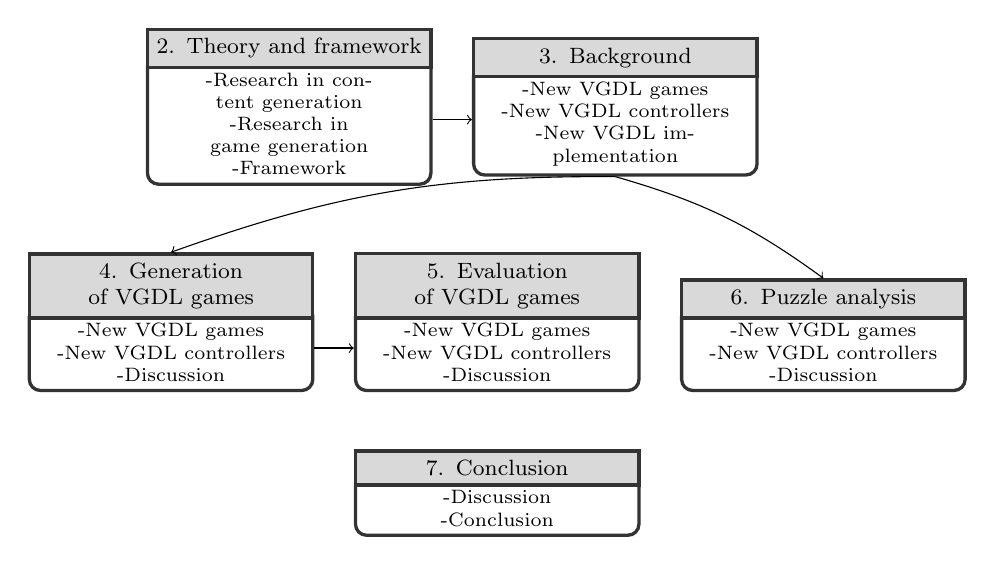
\begin{tikzpicture}[
chapterparts/.style={rectangle, draw=black!80, very thick, text width=3.4cm, font = \scriptsize,inner xsep = 0.1cm,rounded corners},
chapterheader/.style={rectangle, draw=black!80, fill=black!15, very thick, text centered, text width=3.4cm, font = \footnotesize,inner xsep = 0.1cm,},
roundnode/.style={circle, draw=green!60, fill=green!5, very thick, minimum size=7mm},
squarednode/.style={rectangle, draw=red!60, fill=red!5, very thick, minimum size=5mm},
nodes = {align = center}
]
%Nodes

\node[chapterparts]      (theory)
									{\quad\\-Research in content generation\\
									-Research in game generation\\
									-Framework};
\node[chapterparts]      (background) [right=of theory, shift = (left:0.5cm)]
									 {\quad\\-New VGDL games\\
									-New VGDL controllers \\
									-New VGDL implementation};
\node[chapterparts]      (task1) [below=of theory, shift = (left:1.5cm), yshift=-0.5cm]
									 {\quad\\-New VGDL games\\
									-New VGDL controllers \\
									-Discussion};
\node[chapterparts]      (task2) [right=of task1, shift = (left:0.5cm)]
									 {\quad\\-New VGDL games\\
									-New VGDL controllers \\
									-Discussion};
\node[chapterparts]      (task3) [right=of task2, shift = (left:0.5cm)]
									 {\quad\\-New VGDL games\\
									-New VGDL controllers \\
									-Discussion};
\node[chapterparts]      (conclusion) [below=of task2]
									 {\quad\\-Discussion\\
									-Conclusion};
\node[chapterheader]   (theoryh)  [above=of theory, shift = (down:1.2cm)]		
{2. Theory and framework};
\node[chapterheader]   (backgroundh)  [above=of background, shift = (down:1.2cm)]		
{3. Background};
\node[chapterheader]   (task1h)  [above=of task1, shift = (down:1.2cm)]		
{4. Generation of VGDL games};
\node[chapterheader]   (task2h)  [above=of task2, shift = (down:1.2cm)]		
{5. Evaluation of VGDL games};
\node[chapterheader]   (task3h)  [above=of task3, shift = (down:1.2cm)]		
{6. Puzzle analysis};
\node[chapterheader]   (conclusionh)  [above=of conclusion, shift = (down:1.2cm)]		
{7. Conclusion};

%Lines
\draw[->] (theory.east) -- (background.west);
\draw[->] (background.south) to[bend right=10] (task1h.north);
\draw[->] (background.south) to[bend left=10] (task3h.north);
\draw[->] (task1.east) -- (task2.west);

\end{tikzpicture}
\end{center}

\subsection{Terms}
This project is focused a games of two restricted genres and types: 

1) Single-player, 2-dimensional, top-down, action games, in which the player controls a single avatar which can (maximally) be moved in the four cardinal directions, possibly with an "action"-(shoot etc.) button.
These games will be referred to as \textbf{Action-arcade games}.

And: 2) Single-player, 2-dimensional, top-down, turn-based puzzle games, in which the player controls a single avatar which can (maximally) be moved in the four cardinal directions, possibly with an "action"-(shoot etc.) button., and all events occur as a result of player actions (i.e. no NPC's or falling boulders). 
This type of games will be referred to as \textbf{Puzzle games} in the project.

%------------------------------------------------------------------------------------------------------------------------------%
%------------------------------------------------------------------------------------------------------------------------------%
%------------------------------------------------------------------------------------------------------------------------------%
\chapter{Existing research and framework}
\label{ch_existingresearch}
In this chapter we describe the existing research on the topic of procedural content generation (PCG) for games, and specifically game- and level-generation, which is of relevance to the project.
Additionally the framework used for game- and level-generation, and testing is described thoroughly.



\section{Content generation}
\label{sec_contengen}
Before discussing generation of complete games, the research on procedural content generation (PCG) for games are investigated. 
The task of PCG is to create elements for specific parts of a game, for instance levels, weapons, environments, textures and sounds. 
\citet{hendrikx2013procedural} proposes a layered taxonomy to describe PCG of different depths in games, while performing a survey of different ways in which PCG has been implemented in commercial games, noticing that some layers has not been thoroughly explored.

Several different approaches are used in PCG (both in commercial games and in research), however the "search-based" approach (explored by \citet{togelius11search}, \citet{pcgbook:ch2}) dominates the problem.
In search-based generation a \textit{fitness function} is used to score generated content by their quality, making it possible to ensure a high quality of the generator, by either simply generating a large amount of content and choosing the best, or using an evolutionary strategy to evolve better content.




\subsection{Game-level generation}
Almost all video games are highly dependent on designed level or map (or levels/map) in which the game play takes place. Levels are often responsible for creating increasingly challenging situations, and thereby entertaining game play. Super Mario would be way less interesting if enemies and platforms were spread randomly across each level, which would almost certainly result in the game being ether too easy or too difficult.

Several scientific projects have focused on the topic of level-generation with an array of different approaches, some requiring player-input, or simply a helper for human level-designer.

In addition to the other game genres mentioned above, a lot of work has been done in generating levels for puzzle games (ie. Sokoban and Cut The Rope).
Most of the work is focused on generating levels for single game, where some attempt to create general level generation procedures.


\subsection{Other uses of PCG}
Other games have been published applying PCG in different ways. In \textit{Borderlands 2} \citeyearpar{game:borderlands} the player have access to an extreme amount of different weapons, designed by automatic generation.


\subsection{Advantages and disadvantages using PCG}

Having a procedure for generating content in games has a number of advantages:

\begin{itemize}
  \item Content generation allows games to potentially have an endless amount of possibilities, often resulting in higher re-play value than linear games. 
  \item PCG can help game designers generate game levels, often simply by letting the designer explore possible layouts, add decorations or finishing up human-designed levels.
\end{itemize}

PCG also has some problems for generating content for levels:

\begin{itemize}
  \item Generated content can have a feeling of being unauthentic and/or too random. For instance, the positions of decorations in a level (barrels, paintings etc.) can be important for humans, while they are not for computers.
  \item In games where the player follows a story it can be difficult to automatically generate levels, that follow what the game designer intend to happen%.
\end{itemize}




\section{Game generation}
\label{sec_gamegen}
Generating complete games through algorithms is a problem that is being increasingly researched, but work has been done on the topic for last decade. Because the problem is in general quite large, a subset of the problem is usually handled: Only generating certain types of games-, or using different (restricted) frameworks. 
Video games may consist of a large number of tangible and intangible components, including rules, graphical assets, genre conventions, cultural context, controllers, character design, story and dialog, screen-based information displays, and so on~\citet{cook2014angelina,liapis2014creativity,nelson2007automated}.

In this project we look specifically at generating the game-play and -setting of games, i.e. defining a set of game-rules and -objects, and specifying the levels in which the game-play takes place.
The two main approaches that have been explored in generating game rules are reasoning through constraint solving~\citet{smith2010variations} or search through evolutionary computation or similar forms of stochastic optimisation~\citet{togelius2008experiment,browne2008automated,font2013towards}. 
In either case, rule generation can be seen as a particular kind of procedural content generation~\citet{pcgbook:ch6}.

%The idea of generating complete games through algorithms is not itself new. The problem in full generality is quite large, so usually a subset of the general problem is tackled. Videogames may be comprised of a large number of tangible and intangible components, including rules, graphical assets, genre conventions, cultural context, controllers, character design, story and dialog, screen-based information displays, and so on~\citet{cook2014angelina,liapis2014creativity,nelson2007automated}.

%In this paper we look specifically at generating game rules; and more specifically the rules of arcade-style games based on graphical movement and local interaction between game elements, represented in the game description language VGDL. The two main approaches that have been explored in generating game rules are reasoning through constraint solving~\citet{smith2010variations} or search through evolutionary computation or similar forms of stochastic optimisation~\citet{togelius2008experiment,browne2008automated,font2013towards}. In either case, rule generation can be seen as a particular kind of procedural content generation~\citet{pcgbook:ch6}.

It is clear that generating a set of rules that makes for an interesting and fun game is a hard task. 
The arguably most successful attempt so far, Browne's Ludi system, managed to produce a new board game of sufficient quality to be sold as a boxed product~\citet{browne2008automated}. 
However, it succeeded partly due to restricting its generation domain to only the rules of a rather tightly constrained space of board games. 
A key stumbling block for search-based approaches to game generation is the fitness/evaluation function. 
This function takes a complete game as input and outputs an estimate of its quality. Ludi uses a mixture of several measures based on automatic playthrough of games, including balance, drawishness and outcome uncertainy.
These measures are well-chosen for two-player board games, but might not transfer that well to video games or single-player games, which have in a separate analysis been deemed to be good targets for game generation~\citet{togelius2014characteristics}. 
Other researchers have attempted evaluation functions based on the learnability of the game by an algorithm~\citet{togelius2008experiment} or an earlier and more primitive version of the characteristic that is explored in this paper, performance profile of a set of algorithms~\citet{font2013towards}.

A typical approach for generating complete games is searching in a space of possible games. This basically requires two things: That the ratio of enjoyable games in the set is not too low - otherwise those games might never be found. To increase this ratio a game description language (GDL) is often used (searching through all possible Java or C programs would lead to an enormous amount invalid games).
Also, to search through a set of games it is necessary to be able to calculate a fitness value for each game, valuing how enjoyable the game is.


\subsection{Something to note: Levels}
\label{ssec_notelevels}
The problem of generating complete games is heavily linked to the problem of generating levels since most games are deeply tied to the geometry and object-placement defined in levels.
A part of the success of Ludi stem from the fact that levels (boards) were as much in focus, as the game-rules themselves.





\section{Framework: VGDL and the GVG-AI framework}
\label{sec_gvgaiframework}
Regardless of which approach to game generation is chosen, one needs a way to represent the games that are being created.\footnote{See \citet{pcgbook:ch6} for a discussion of game-rule representation choices.} For a sufficiently general description of games, it stands to reason that the games are represented in a reasonably generic language, where every syntactically valid game description can be loaded into a specialised game engine and executed. 
There have been several attempts to design such GDLs. One of the more well-known is the Stanford GDL, which is used for the General Game Playing Competition~\citet{genesereth2005general}. That language is tailored to describing board games and similar discrete, turn-based games; it is also arguably too verbose and low-level to support search-based game generation. 
Another attempt at an VGDL is called PuzzleScript, created by game designer Stephen Lavelle. The language (as its name suggest) is focused on turn-based puzzle games, but the engine allows for simple forms of animation and movement. The language is relatively high level compared to Stanford GDL, but does not support that large set of video games.


\subsection{VGDL game description}
\label{ssec_vgdl}
The various game generation attempts discussed above feature their own GDLs of different levels of sophistication; however, there has not until recently been a GDL for suitably for a larger space of video game types- and genres.
The Video Game Description Language (VGDL) is a GDL designed to express 2D arcade-style video games of the type common on hardware such as the Atari 2600 and Commodore 64. It can express a large variety of games in which the player controls a single moving avatar (player character) and where the rules primarily define what happens when objects interact with each other in a two-dimensional space. VGDL was designed by a set of researchers~\citet{levine2013general,ebner2013towards} (and implemented by Schaul ~\citet{schaul2013video}) in order to support both general video game playing and video game generation.
In contrast to other GDLs, the language has an internal set of classes, properties and types that each object can defined by, which the authors suggest the user to extend.

Objects have physical properties (i.e. position, direction) which can be altered either by the properties defined, or by interactions defined between specific objects. 
Playing the games also required a specified level which defines a set of game-tiles deciding the initial locations of sprites. When running games sprite can move in between game-tiles (if the \textbf{speed} is a fraction).

A VGDL description has four parts: 

\begin{description}
\item [SpriteSet] Defines which sprites can appear in the game. Each sprite must be designated by a class, in which a set of predefined actions exists. Also a set of parameters can be fed to each sprite, configuring for instance the speed or how often the sprite takes an action, and the parameters used for the different sprite-classes -- for instance, for the  class \textbf{Flicker} (a simple extension to the base sprite, the sprite is destroyed after a speecifed amount of time) the lifetime can be adjusted.
Sprites can additionally be designed in a tree structure, where multiple sprites have the same parent sprite, making more possibility for the interactions and terminations described below. 
\item [InteractionSet] Each line defines what happens when a set of two sprites collide with each other (located on the same game-tile). Each interaction is represented by a class defining the action to take (i.e. push back, or kill sprite), and a set of parameters specific to each interaction-class, as well as the score achieved for letting the interaction happen.
\item [TerminationSet] Defines how the game can end. Each line in this set has a win parameter, which is set to true or false; winning or losing the game.
Each termination-function is represented by a class defining under which conditions the game should end, which can for instance when there exists 0 of a certain sprite (when all of the sprites are killed).
\item [LevelMapping] The job of the \texttt{LevelMapping} is to translate from a character (\texttt{char}) in a level-file (explained below), to sprites from the \texttt{SpriteSet}. 
A single mapping can be shared by several sprites, causing the sprites to be created on the same game-tile.
\end{description}



\begin{figure}[!ht]
\centering
\begin{vgdldesc}[linewidth=14cm]
BasicGame
	SpriteSet
		city  > Immovable color=GREEN img=city
		explosion > Flicker limit=5 img=explosion
		movable >
			avatar  > ShootAvatar stype=explosion
			incoming >
				incoming_slow  > Chaser stype=city color=ORANGE speed=0.1
				incoming_fast  > Chaser stype=city color=YELLOW speed=0.3

	LevelMapping
		c > city
		m > incoming_slow
		f > incoming_fast
		
	InteractionSet
		movable wall  > stepBack
		incoming city > killSprite
		city incoming > killSprite scoreChange=-1
		incoming explosion > killSprite scoreChange=2

	TerminationSet
		SpriteCounter stype=city   win=False
		SpriteCounter stype=incoming win=True
\end{vgdldesc}
\caption{Example of VGDL description - a simple implementation of the game Missile Command}
\label{fig:vgdlgame}
\end{figure}

Additionally each game can only be played using level files. 
A level file is written using the \texttt{LevelMapping} characters, where each character defines a tile of the game, and spaces defines empty tiles.

\begin{figure}[!ht]
\centering
\begin{vgdldesc}[linewidth=14cm]
w    m  m   m  m  m m mw
w                      w
w                      w
w                      w
w                      w
w                      w
w           A          w
w                      w
w                      w
w                      w
w   c c c c c c c c    w
wwwwwwwwwwwwwwwwwwwwwwww
\end{vgdldesc}
\caption{Example of VGDL level description - a level for the implementation of the game Missile Command}
\label{fig:vgdlgame_level}
\end{figure}



\subsection{The GVG-AI framework: AI controllers and testing}
\label{ssec:aicontrollersandtesting}
The GVG-AI framework is a testbed for testing general game-playing controllers against games specified using VGDL. Controllers are called once at the beginning of each game for setup, and then once per clock tick to select an action. Controllers do not have access to the VGDL descriptions of the games. They receive only the game's current state, passed as a parameter when the controller is asked for a move. However these states can be forward-simulated to future states. Thus the game rules are not directly available, but a simulatable model of the game can be used.

\subsubsection*{GVG-AI sample controllers}
The GVG-AI contains a series of sample AI controllers, which some were used in testing games in the project.
Below is a short description of each of the sample controllers used:

\begin{description}
	\item [MCTS] ``Vanilla'' MCTS using UCT.
	\item [GA] Uses a genetic algorithm to evolve a sequence of actions.
	\item [OneStep-Heuristic] Heuristically evaluates the states reachable through one-step lookahead. The heuristic takes into account the locations of NPCs and certain other objects.
    \item [Random] Chooses a random action from those available in the current state.
\end{description}

\subsubsection*{GVG-AI example games}
The framework additionally contains 20 hand-designed games, which partly consist of interpretations of classic video games (e.g. Boulderdash, Frogger, Missile Command and Pacman), while some are original creations by the General Video-Game AI Competition's organizers. 
Note however, that the interpretations of class games all have different stages of simplifications to them, causing several of the games' features to be missing -- for instance, the player cannot push boulders in the VGDL version of Boulderdash and they do not "roll" as in the original, and the ghosts in Pacman behave in a much more simplified fashion.
A short summary of each of the example games can be seen in Appendix \ref{app_gvgaigames}

The games can be described (except for the game \emph{Sokoban}) as \textit{action-arcade} games, in that the player controls a single avatar which must be moved quickly around in a 2D-setting to win, or to get a high score (the player is able to increment a score  counter in all of the games).
Figure \ref{fig:vgdlgame} shows the VGDL description of the game \emph{Missile Command}, and \ref{fig:vgdlgame_level} a level description from the same game.




\begin{figure}[!ht]
	\subfloat{%\emph{Zelda}\label{subfig-2:dummy}]{%
      		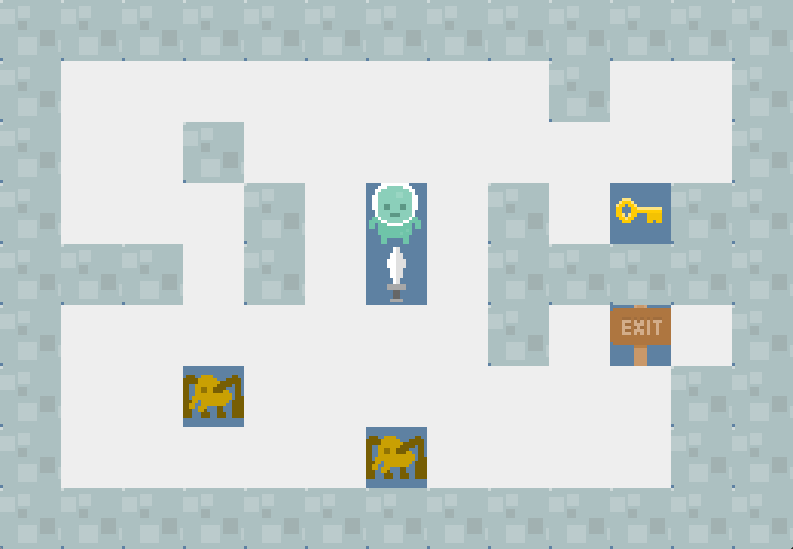
\includegraphics[scale=0.18]{zelda.png}
    	}
	\hfill
	\subfloat{%[\emph{Portals}\label{subfig-1:dummy}]{%
		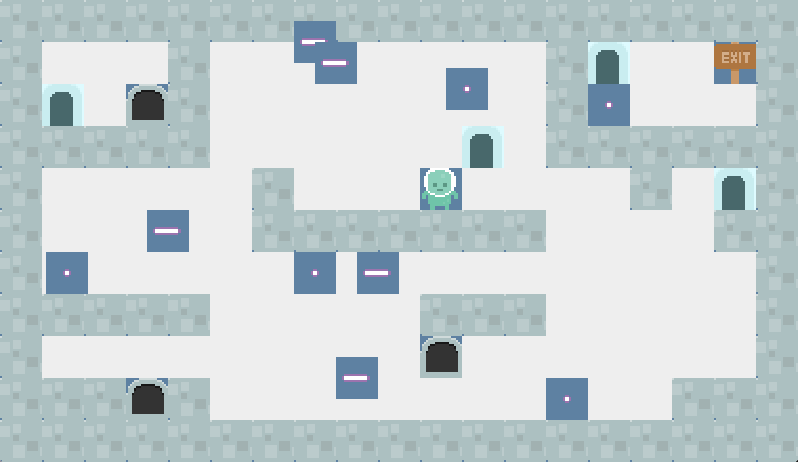
\includegraphics[scale=0.24]{portals.png}
	}\\
	\subfloat{%\emph{Boudlerdash}\label{subfig-2:dummy}]{%
      		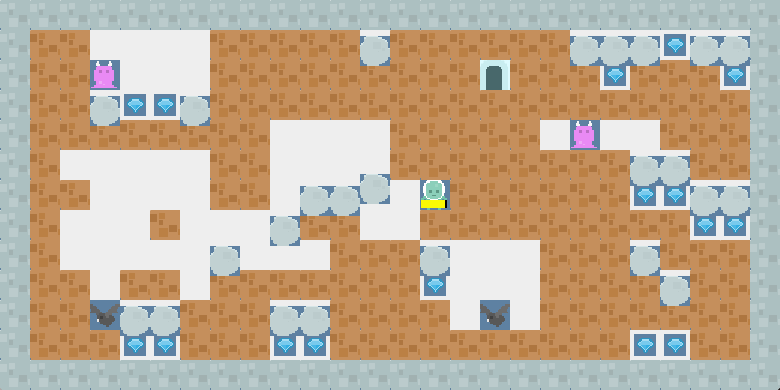
\includegraphics[width=\textwidth]{boulderdash.png}
    	}
    	\caption{A visual representation of a few of the VGDL example games. From top-left: \emph{Zelda}, \emph{Portals} and \emph{Boulderdash}}
	\label{fig:dummy}
\end{figure}





\subsubsection*{Restrictions of VGDL and the GVG-AI framework}
\label{ssec_gamegenres}
The VGDL implementation of the GVG-AI competetion is essentially (without great extension) only able to describe certain action-arcade games, and puzzle games.
For instance, the lack of possibility to traverse different levels make \textbf{Adventure} games impossible to make, and the restriction of only being able move a single character with the keyboard (the avatar) makes great restriction in creating \textbf{Strategy} games.

In this project we will focus on the two main type of games describable in VGDL: Action-arcade games and turn-based puzzle games. We make the simple distinction that arcade games contain elements (sprites) that move by themselves, whereas interactions only occur as a result of the avatar moving in puzzle games.
This puts the game \emph{Portals} in the arcade genre, even though it contains puzzle elements.









%------------------------------------------------------------------------------------------------------------------------------%
%------------------------------------------------------------------------------------------------------------------------------%
%------------------------------------------------------------------------------------------------------------------------------%

\chapter{Extending VGDL}
\label{ch_extending}
This chapter describes a series of extensions we constructed for VGDL and the GVG-AI framework, making a more in-depth analysis possible.
We created a series of VGDL games, AI controllers and a implemented a new, simplified framework to play through \textit{puzzle games} with less time and memory use.


\section{Writing new VGDL games}
\label{sec_writingnewvgdl}
To increase the size of the set of designed games, to allow for a more precise analysis of what makes a game "good", we created fourteen new game descriptions in VGDL. 

Another important reason for creating new descriptions, was to introduce a series of \emph{puzzle games} to be analysed, since, as mentioned in Section \ref{ssec_vgdl} the example games from the GVG-AI competetion are almost all \textit{action-arcade} games.


\subsection{Describing existing games in VGDL}
The main goal when developing a game - which also applies in this case - is to ensure that it is enjoyable to human-players. 
Therefore the games implemented are all interpretations of published existing games (and not original creations).
As described in \textbf{Section \ref{ssec_gamegenres}} VGDL can only describe relatively simple games of certain types/genres, and so only a limited number of games can be translated without severely changing the game-play.

The games we created, and described below are in general "exact" copies of the originals - containing all the game-play features and interactions but lacking elements like audio, graphics and controls. 
However many lack certain (non-essential) game-play features like bonus points (like fruits in Pac-Man), infrequently appearing enemies (UFOs in Space Invaders) or features which only appear in some levels of the games.


\subsection{Results}
A series of fourteen commercial games was re-created in VGDL to be used in future tests. 
Figure \ref{fig:centipedeTranslation} shows one of the games translated to VGDL.
Minor changes to the GVG-AI framework was made for a small number of the games, to be able to correctly copy the games' core gameplay features.
The original game levels were additionally translated into VGDL level description, with five levels being created for each game.
For some of games the levels could not be completely copied, for instance because the levels were too large in size (\textit{Bolo Adventures}), or because a lack of game features implemented in the clones (\textit{Chip's Challenge}), and the resulting levels are therefore simplifications of the originals..

\subsubsection*{Action-arcade games}
A set of four Atari -arcade and -2600 games were found to be suitable for interpretation; \textit{Solar Fox}, \textit{Crackpots}, \textit{Centipede} and \textit{Astrosmash}, and a VGDL game description was written for each. 
A description of each of the games and their interpretations can be seen in Appendix \ref{app_thesisgames}

\begin{figure}[!ht]
${\vcenter{\hbox{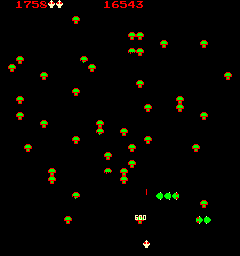
\includegraphics[height=6cm]{origcentipede.png}}}} \vcenter{\hbox{\scalebox{2}{\Huge\pointer}}}
\vcenter{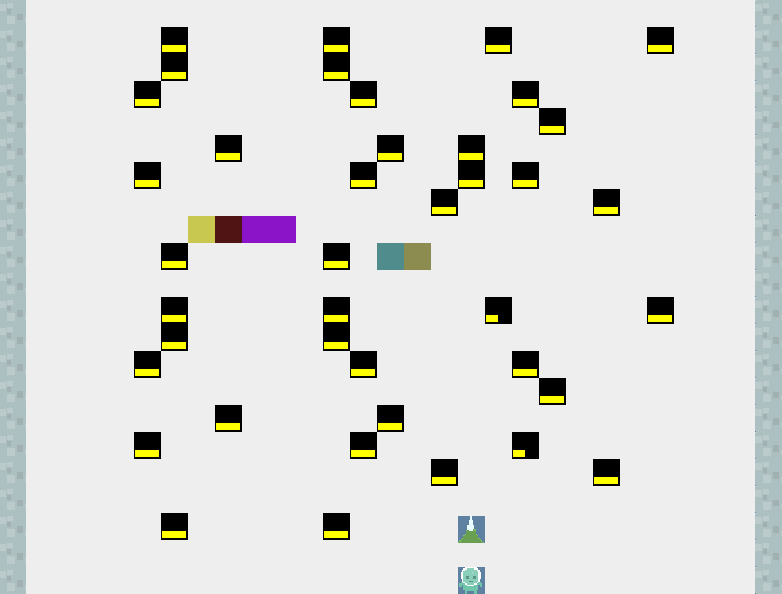
\includegraphics[height=6cm]{vgdlcentipede.png}}
$
    	\caption{Interpretation of the classic arcade game \textit{Centipede} \citeyearpar{game:crackpots}}
\label{fig:centipedeTranslation}
\end{figure}


\subsubsection*{Puzzle games}
A set of puzzle games from several different platform, all featuring a single avatar, was found to be suitable to be described in VGDL. 
Several of these games can be described as \textit{Sokoban}-clones with different spins on the gameplay.
The games interpreted were \textit{Sokoban}, \textit{Bait}, \textit{Bombuzal}, \textit{Bolo Adventures}, \textit{Zen Puzzle}, \textit{The Citadel}, \textit{Brainman}, \textit{Chip's Challenge}, \textit{Modality} and \textit{Painter}.





%------------------------------------------------------------------------------------------------------------------------------%

\section{Creating new VGDL controllers}
\label{sec_creatingnewcontrollers}
To be able to probe VGDL games in more detail, we created a series of new AI controllers with various approaches to finding a results.
In total five new controllers was generated: Three to play the action-arcade style games, and two only focused on puzzle games.

\subsection{Action-arcade controllers}
\label{ssec_actioncontrollers}

Three controllers of an increasing degree of cleverness was introduced: \textit{One-step} (least clever), \textit{Deep-search} and \textit{Explorer} (most clever). 
The controllers greatly differ in their strategy in simulating the forward model (accessible when running the GVG-AI framework) using different actions, and different series of actions.

\subsubsection*{One-step}
The One-step AI only attempt to advance the forward model once, for each allowed action in the game.
The score and win/lose state of the resulting game states are then considered, and the action with the resuling best state is chosen -- and a random action is chosen when no state is better than others.
The controllers approach can be seen below:

\begin{algorithm}[H]
\For{action : PossibleActions}{
newGameState = gameState.copy().advance(action) \\
value[action] = value(newGameState) \\
}
\Return action leading to highest value, or random action if values are equal
\end{algorithm}

\subsubsection*{Deep-search}
This controller starts out in a similar fashion as the One-step, by expanding using all possible actions by copying the initial game-state.
These game-states are then simulated further upon by advancing each game state a single time, with a random action, without copying the state (a rather costly procedure).
This expansion is continued until the controller runs out of time, and a value for each action is calculated by considering the score and win/lose-value for each state that can be achieved from each of the initial states.

\begin{algorithm}[H]
queue $\gets$ initial gameState \\
\While{has time left}{
	gameState = q.poll() \\
	\eIf{gameState == initial gameState}{
		\For{action : PossibleActions}{
			queue $\gets$ gameState.copy().advance(action)
		}
	}{
		gameState.advance(random action) \\
		d $\gets$ depth of search (amount actions performed) \\
		value[action] $+=$ value(newGameState) $* \text{PossibleActions.length}^{\text{d}}$
	}
}
\Return action leading to highest value, or random action if values are equal
\end{algorithm}

\subsubsection*{Explorer}
The explorer controller was designed specifically to play the arcade-style games of the GVG-AI framework, and utilizes a series of methods to strengthen its decisions. 
Unlike the other controllers which utilise open-loop searches, it stores information about visited tiles and prefers visiting unvisited locations. 
Overall the controller uses three different arrays to choose an action: One considering how probable death is from each action, one examining the score that can be achieved from the actions, and one only looking at the boringness.
If the \textit{death}-array have too high values, that array is used to take the decision (the action leading to the lowest value is chosen), otherwise the best action from the score-array is used.
If the values of the \textit{score}-array happen to be too similar, the \textit{boringness}-array is lastly used instead.

The controller also addresses a common element of the VGDL example games, randomness. The controller gains an advantage in many of the games by simulating the results of actions repeatedly, before deciding the best move.

The Explorer was proven to be of a decent quality by getting a 2nd / 7th place in the GVG-AI competition. SOURCE

\subsection{Puzzle controllers}

\subsubsection*{Breadth first}

\subsubsection*{Best first}


%------------------------------------------------------------------------------------------------------------------------------%

\section{FastVGDL}
\label{sec_fastvgdl}
Since the GVG-AI framework has some functions and properties which are not interesting for some parts of this work, we created an implementation of a lighter version of VGDL, solely focused on analysing puzzle games in more detail.
The implementation is basically a clone of the GVG-AI framework, but with several time- and memory consuming features removed, which in part was possible due to the puzzle games being relatively more simple (for instance, only movement from one tile to another is possible in FastVGDL, whereas sprites can move and collide in-between tiles in the GVG-AI framework).

SMALL TEST SHOWING TIME AND MEMORY DIFFERENCE PL0X!!!

 


%------------------------------------------------------------------------------------------------------------------------------%
%------------------------------------------------------------------------------------------------------------------------------%
%------------------------------------------------------------------------------------------------------------------------------%

\chapter{Automatic generation of VGDL descriptions}
\label{ch_task1autogenofvgdl}
This chapter describes the setup- and methodology used in generating new games (i.e. game descriptions).
Additonally an initial play test of set of both human-designed and generated games, using an array of different AI-controllers explained in the previous chapters.

This chapter is only focused on \textit{action-arcade} games - \textit{puzzle games} will be discussed and analysed in Chapter \ref{ch_puzzles}.

\subsubsection*{Selected designed arcade-action games}
A subset of the human-designed games mentioned in Section \ref{sec_gvgaiframework} and \ref{sec_writingnewvgdl} were selected for the following analyses games, and for creating new games by mutation.

After our addition of new games to GVG-AI framework we have access to 34 games, with five levels each. 
However, only 23 of the games are of the \textit{arcade-action} genre explored in this section. 
Additionally, as mentioned in Section \ref{ssec_vgdl} a few of the example games from the GVG-AI competition are original creations, which cannot equally be assumed to be human-enjoyable.

With these limitation, thirteen interpretions of existing games are left and used as a baseline for testing and game generation: Aliens, Boulderdash, Frogs, Missile Command, Zelda, DigDug, Pacman, Seaquest, Eggomania, Solar Fox, Crackpots, Astrosmash and Centipede.

A slight change was also made to the GVG-AI framework, removing the possibility of players scoring lower than 0, which is the norm in the original games mentioned (this also makes comparing scores more straightforward).


%        games = new String[]{"aliens", "boulderdash", "butterflies", "chase", "frogs",
%                "missilecommand", "portals", "sokoban", "survivezombies", "zelda",
%                "camelRace", "digdug", "firestorms", "infection", "firecaster",
%                "overload", "pacman", "seaquest", "whackamole", "eggomania"};

%non-orignal action-arcade: aliens, boulderdash, frogs, missilecommand, zelda, digdug, pacman, seaquest, eggomania


\section{Generating processes}
\label{sec_task1genApproach}
Using the GVG-AI framework described in Section \ref{sec_gvgaiframework} we constructed a setup for generating large sets of new game description.
We used two different approaches in generating new game description in VGDL: Mutating existing (designed) games, and randomly generating games from scratch.
In both approaches several constraints were set upon the generation process to prevent crashes, and to increase the chance of a human playable game.



\subsection{Mutation of example games}
\label{ssec_task1mutation}
A process was built for parsing existing VGDL game descriptions, mutating certain sprites- or rules, and returning new, valid game descriptions,.
The set of games described at the beginning of this chapter, were chosen to be used as a basis for mutating new game descriptions, analysed in this section.



\subsubsection*{Generating approach}
It is not immediately apparent which approach to use in mutating the different elements of  each VGDL game description.
Since sprite- and rules are constructed from a combination of a class and a series of parameters specific to the class, it is necessary to change the parameters if the class is changed, but the parameters of an existing class can freely be mutated.

A process was built for mutating each of the different parts of game descriptions, i.e. changing the sprites available of the \texttt{SpriteSet}, the interactions rules (\texttt{InteractionSet}) and the termination rules (\texttt{TerminationSet}).
The process additionally allowed for changing the amount of rules, i.e. generating new rules or removing existing ones.

Since the sprites and rules of each game description is described by both a class and a series of parameters, several partly subjective decisions was made on defining probabilities of different parameters' values to try reach "realistic" values.
For instance it was decided that a sprite being mutated or generated only has a 25\% chance of using the \texttt{cooldown} parameter (making sprites have pauses between acting), and that the parameter have a random value between 1 and 10.
The values and probabilities used were mostly decided by examining the set of designed games descriptions.
Several constraints were also used to avoid game with non-valid descriptions (which can cause crashes in the GVG-AI framework), for instance by ensuring that avatar-sprites cannot be spawned and sprites cannot transform to an avatar, but an avatar sprite can still transform to another type of avatar sprite.

In this work we decide to only mutate interaction-rules from the \texttt{InteractionSet} of designed VGDL games, and simply change every part (classes, parameters and references) of a random amount of rules, with each rule having a 25\% change of being changed for each game to mutate.
In addition to simplifying the mutation process, and having games more with a higher chance of being playable this allows us to use the original designed games' levels for testing.

%When testing mutated games the original games' levels were used. Therefore the amount of sprites and the \texttt{LevelMapping} was not changed.


EXAMPLE OF MUTATED GAME --- GAME DESCRIPTION ANDOR SCREENSHOT


\subsection{Random game generation}
\label{ssec_task1rndGen}
A similar process as mentioned above was used to randomly put game descriptions together creating new games completely from scratch, constructing the textual lines for different parts of a VGDL description: Generating an array of sprites (for the SpriteSet), interaction-rules (InteractionSet), termination-rules (TerminationSet) and level mappings (LevelMapping). 

Several partly subjective choices were again made for the range for the amount of different sprites, and interaction- and termination rules. 
Even though some of the original games contain a larger set of elements, we constricted the ranges to sprites: ${3-8}$, interactions: ${3-10}$ and terminations: ${2}$ (a "win-" and a "lose"-termination).


When generating descriptions, we used similar constraints to those mentioned in section~\ref{method:mutation}, partly to avoid generating descriptions with invalid elements, and partly to increase the proportion of interesting outcomes. 
As for the mutated games, some partly subjective decisions were made on defining the possible amount of sprites and rules, the proportion of sprites that has a level mapping, and when generating new sprite definitions.

To simplify the sprite creation process, no parent-child structure was used in the \texttt{SpriteSet}.
However, the goal of the parent-child structure is only to make rule definitions less verbose, and does not make actual new game features possible.


%\begin{figure}[ht]
%	\centering
%	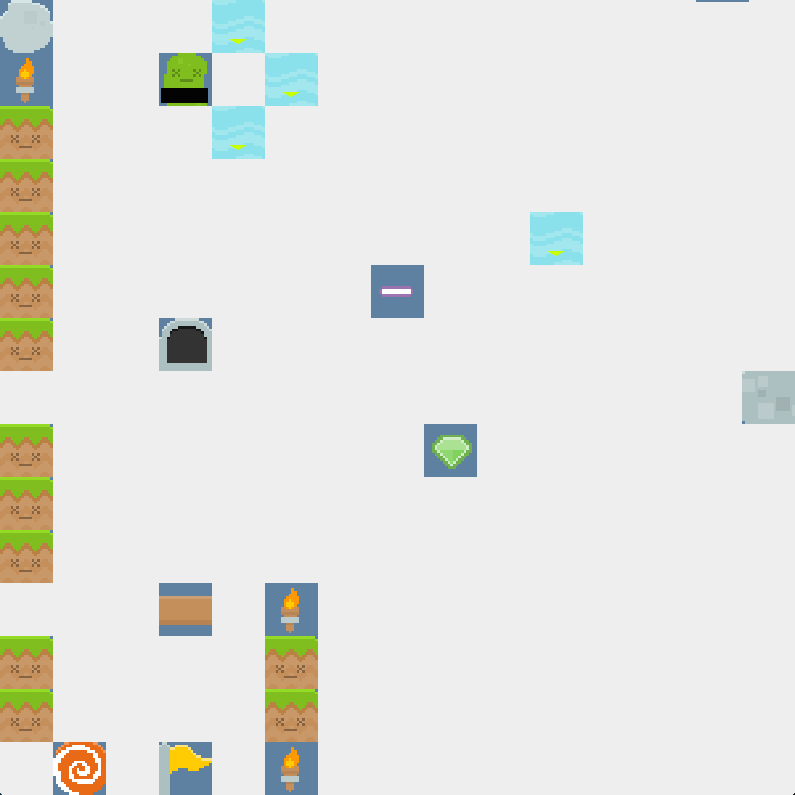
\includegraphics[width=0.45\textwidth]{gengame.png}
%	\caption{Visual representation of one of the 400 randomly generated VGDL games}
%\end{figure}


\subsubsection*{Level generation}
As mentioned in Section \ref{ssec_notelevels} the problem of generating a game is more often than not intimately linked to a generation of levels.
I.e. we could end up with generating game descriptions of high quality games, but if the level descriptions does not fit to the game-play (by being too trivial, or too hard for instance) the games might not found if searching through a set of randomly generated games.

A simple level generator were constructed with the simple goal of making the randomly generated games playable.
The generator designates a level built using a given size, and inserts sprite mappings in different positions which takes all the level mappings from a game description and put a random (but small) amount of each sprite defined, in random location(s).




%------------------------------------------------------------------------------------------------------------------------------%

\section{Initial test: Experimental setup}
\label{sec_task1inittestsetup}
In this section we present a set of initial results from playing through both designed and generated games using different AI controllers, and discuss different ways to analyse the resulting data.


\subsubsection*{Controllers}
Eight general videogame controllers were used to test the games. The controllers use different approaches, with a varying degree of intelligence. Four of the controllers are included in the GVG-AI framework, while the remaining were implemented for this work. Except for \emph{OneStep-Heuristic}, the controllers only evaluate a given state according to its score and win/loss status.
Each controller was marked with one of four types of intelligence for later tests: Intelligent (complex searches in game space are taken), semi-intelligent (game space search uses simple approach), random and do-nothing.


\subsubsection*{Generated games}
A set of XXX mutated games were generated, by mutating each of the designed games ten times using the approach described in the previous section.
400 randomly generated games, each with a single generated level attached, were additionally developed and used in testing.

\subsubsection*{Testing and result analysis}
The eight controllers were used to play through different set of example-, mutated and randomly generated games. Because of CPU budget limitations, each game was played with a maximum amount clock ticks of 800, and each controller was restricted to use 50 ms on each tick. 
For each playthrough only the default data from the GVG-AI framework was retrieved: The \textit{score}, the \textit{win-lose value}, the amount of \textit{clock ticks} used and a list of actions performed.



A process to analyse the data was built, to calculate averages, standard deviations, max-, minimum and other statistics of each of the values, for each controller, with the possibility of calculating averages across several levels or games.
To more accurately compare the \textit{score} for the different controllers when playing across a range of different games  we additionally calculate a normalised score using a max-min normalisation. 
The entropy of actions performed was also calculated, again with an average over all play throughs- or games.

Each game was played through 25 times, all within a single level attached to the game.


\section{Initial test: Results}
\label{sec_task1inittestresults}
 
In this section we show results of the tests explained above, analyse the average of all play-throughs for each controller, and compare the results with each other.
Before analysing and presenting the data, for all of the below tests we first remove games from the set which we consider either too difficult to analyse, or too simple too possibly be of interest -- namely we remove games by three different considerations: 
1) When a controller was disqualified (too many sprites- and/or interactions happening), 2) where the standard deviation of score was zero for all controllers, and 3) where the game always end in less than 50 clock ticks (which is the maximum lifetime of generated \texttt{Flicker}-sprites).

\subsubsection*{Designed games}
The eight controllers were set to play through each of the human-designed VGDL games, with the constraints mentioned above.

We present the averages across each single game(can be seen in Appendix \ref{app_designedresults}) and averages across all of the games, seen in Figure \ref{table:designed}.
The distributions show that more intelligent controllers tend to have more success, with both a higher win-rate and a significantly higher average score. 
The \textit{clock-ticks} and \textit{action entropy} does not show any similar distribution for the collection of all games. 
Examining the results from each game it is noticeable that the profiles for these values (\textit{clock-ticks} and \textit{entropy}) are very different from game to game.

It should be noted that the uncertainties for average score, clock-ticks and action entropy assume a normal distribution of the data which in general is not true, and so these values should be taken with a grain of salt.

\begin{figure}[!ht]
\centering
\csvreader[tabular=lrrrrr,
    table head=\toprule \textit{\textbf{controller}}
             & \textit{ave. score}
             & \textit{norm. score}
             & \textit{win-rate}
             & \textit{ave ticks}
             & \textit{ave. act entr.},
    late after head=\csvifoddrow{\\\rowcolor{black!5}}{\\\rowcolor{black!25}}\midrule,
    late after line=\csvifoddrow{\\\rowcolor{black!5}}{\\\rowcolor{black!25}},
    late after last line=\\\bottomrule
    ]%
{examplesdata.csv}{1=\Agent,2=\Mean,4=\MeanErr,5=\MMMean,7=\MMMeanErr,8=\WR,9=\WRErr,15=\TicksMean,17=\TicksMeanErr,18=\ActEntMean,19=\ActEntMeanErr}%
{\Agent & \num{\Mean} (\num{\MeanErr}) & \num{\MMMean} (\num{\MMMeanErr}) & \num{\WR} (\num{\WRErr}) & \num{\TicksMean} (\num{\TicksMeanErr}) & \num{\ActEntMean} (\num{\ActEntMeanErr})}%

\caption{Averaged results across all the XX designed games}
\label{table:designed}
\end{figure}


\subsubsection*{Mutated games} 
After removing games by the requirements mentioned above, we were left with a toal of 146 games in which we had useful data.
The results of playing through these games with the controllers can be seen in Figure~\ref{table:mutated}. 
The scores have higher means and standard deviations, indicating outliers in the data. 
The ordering of the \emph{normalised score mean} and \textit{win-rate}, however, shows a similar pattern as for the example games, with Explorer again excelling.

It should be noted here that the differences between the extreme values of \textit{score} and \textit{win-rate} are smaller than for the designed set of games.

%all mutations average -- amount of games: 146 -- playthroughs: 25
\begin{figure}[!ht]
\centering
\csvreader[tabular=lrrrrr,
    table head=\toprule \textit{\textbf{controller}}
             & \textit{ave. score}
             & \textit{norm. score}
             & \textit{win-rate}
             & \textit{ave ticks}
             & \textit{ave. act entr.},
    late after head=\csvifoddrow{\\\rowcolor{black!5}}{\\\rowcolor{black!25}}\midrule,
    late after line=\csvifoddrow{\\\rowcolor{black!5}}{\\\rowcolor{black!25}},
    late after last line=\\\bottomrule
    ]%
{mutateddata.csv}{1=\Agent,2=\Mean,4=\MeanErr,5=\MMMean,7=\MMMeanErr,8=\WR,9=\WRErr,15=\TicksMean,17=\TicksMeanErr,18=\ActEntMean,19=\ActEntMeanErr}%
{\Agent & \num{\Mean} (\num{\MeanErr}) & \num{\MMMean} (\num{\MMMeanErr}) & \num{\WR} (\num{\WRErr}) & \num{\TicksMean} (\num{\TicksMeanErr}) & \num{\ActEntMean} (\num{\ActEntMeanErr})}%

\caption{Averaged results across the 146 mutated games}
\label{table:mutated}
\end{figure}



\subsubsection*{Generated games}
Figure~\ref{table:generated} shows results for the remaining 65 randomly generated games (of 400), with problematic games removed according to the same criteria as in the previous section.

First of all, the \emph{score} have much more extreme values than in the previous games, with the minimum being 199,406.58, over 1500 times larger than the highest in the set of example games (i.e. 121.55, by Explorer).
Clearly, only the \emph{normalised mean} can be used to compare scores across the different controllers. 
The \emph{normalised score means} and \emph{win-rates} both have values that are more closely clustered togther, than in the previous game sets. 
For this set of games the \textit{action entropy} of the intelligent controllers has also fallen quite a bit (relative to the Random-controller), indicating that more of the games have simple solutions to win or increase the score

It should be noted that the description generation process can often end up making games be automatically won (for instance, the goal of a game could be to destroy all coins, but all coins are of the \texttt{Flicker}-class and disappear after a certain amount of time), which causes the relative high \textit{win-rate} for the Do Nothing-controller.

%gengames average -- amount of games: 65 -- playthroughs: 25
\begin{figure}[!ht]
\centering
\csvreader[tabular=lrrrrr,
    table head=\toprule \textit{\textbf{controller}}
             & \textit{ave. score}
             & \textit{norm. score}
             & \textit{win-rate}
             & \textit{ave ticks}
             & \textit{ave. act entr.},
    late after head=\csvifoddrow{\\\rowcolor{black!5}}{\\\rowcolor{black!25}}\midrule,
    late after line=\csvifoddrow{\\\rowcolor{black!5}}{\\\rowcolor{black!25}},
    late after last line=\\\bottomrule
    ]%
{generateddata.csv}{1=\Agent,2=\Mean,4=\MeanErr,5=\MMMean,7=\MMMeanErr,8=\WR,9=\WRErr,15=\TicksMean,17=\TicksMeanErr,18=\ActEntMean,19=\ActEntMeanErr}%
{\Agent & \num{\Mean} (\num{\MeanErr}) & \num{\MMMean} (\num{\MMMeanErr}) & \num{\WR} (\num{\WRErr}) & \num{\TicksMean} (\num{\TicksMeanErr}) & \num{\ActEntMean} (\num{\ActEntMeanErr})}%

\caption{Averaged results across the 65 generated games}
\label{table:generated}
\end{figure}


\subsubsection*{Outcome and graphs}
By examining the graphs (Figure \ref{graph:maxminmean} and Figure \ref{graph:winrate}) of the data just discussed, it is clear that there is a strong relationship between the performance profiles of playing with controllers of different types, on different set of games.
However it should be noted here that some games from both the mutated- and generated game-set, contains games, which when examined by themselves have similar distributions as the average designed game.

\begin{figure}[!ht]
\centering
\begin{tikzpicture}[font=\small, scale=1]
  \begin{axis}[
	ybar, bar width=0.38cm,
	xtick=data, xtick pos=left,
	ylabel=Average normalised score, ymajorgrids, ymin=0, ymax=1,
	symbolic x coords={Explorer,MCTS,GA,Onestep-S,Onestep-H, Random, Do Nothing},
	width=\textwidth, height=6cm,
	legend style={
	  overlay, area legend, anchor=north,legend columns=1, at={(0.913,1.00)} %, at={(0.5,-0.15)}
	},
	legend image code/.code={%
          \draw[#1, draw=none] (0cm,-0.1cm) rectangle (0.6cm,0.1cm);
        }
]
    \addplot[fill=LightBlue, error bars/.cd, y dir=both, y explicit] table [x=Agent:, y=MaxMinN-Mean:, y error=MaxMinN-SE:, col sep=comma] {examplesdata.csv};
    \addplot[fill=LighterBlue, error bars/.cd, y dir=both, y explicit] table [x=Agent:, y=MaxMinN-Mean:, y error=MaxMinN-SE:, col sep=comma] {mutateddata.csv};
    \addplot[fill=LightestBlue, error bars/.cd, y dir=both, y explicit] table [x=Agent:, y=MaxMinN-Mean:, y error=MaxMinN-SE:, col sep=comma] {generateddata.csv};
\legend{examples,mutated,generated}
\end{axis}
\end{tikzpicture}
\caption{Averaged normalised score across all games of the three different set of games: Designed-, mutated- and completely generated games}
\label{graph:maxminmean}
\end{figure}


\begin{figure}[!ht]
\centering
\begin{tikzpicture}[font=\small, scale=1]
  \begin{axis}[
	ybar, bar width=0.38cm,
	xtick=data, xtick pos=left,
	ylabel=Average normalised score, ymajorgrids, ymin=0, ymax=1,
	symbolic x coords={Explorer,MCTS,GA,Onestep-S,Onestep-H, Random, Do Nothing},
	width=\textwidth, height=6cm,
	legend style={
	  overlay, area legend, anchor=north,legend columns=1, at={(0.913,1.00)} %, at={(0.5,-0.15)}
	},
	legend image code/.code={%
          \draw[#1, draw=none] (0cm,-0.1cm) rectangle (0.6cm,0.1cm);
        }
]
    \addplot[fill=LightBlue, error bars/.cd, y dir=both, y explicit] table [x=Agent:, y=Winrate:, y error=Winrate-SE:, col sep=comma] {examplesdata.csv};
    \addplot[fill=LighterBlue, error bars/.cd, y dir=both, y explicit] table [x=Agent:, y=Winrate:, y error=Winrate-SE:, col sep=comma] {mutateddata.csv};
    \addplot[fill=LightestBlue, error bars/.cd, y dir=both, y explicit] table [x=Agent:, y=Winrate:, y error=Winrate-SE:, col sep=comma] {generateddata.csv};
\legend{examples,mutated,generated}
\end{axis}
\end{tikzpicture}
\caption{Averaged win-rate for the three sets}
\label{graph:winrate}
\end{figure}



\begin{figure}[!ht]
\centering
\begin{tikzpicture}[font=\small, scale=1]
  \begin{axis}[
	ybar, bar width=0.38cm,
	xtick=data, xtick pos=left,
	ylabel=Average normalised score, ymajorgrids, ymin=0, ymax=1000,
	symbolic x coords={Explorer,MCTS,GA,Onestep-S,Onestep-H, Random, Do Nothing},
	width=\textwidth, height=6cm,
	legend style={
	  overlay, area legend, anchor=north,legend columns=1, at={(0.913,1.00)} %, at={(0.5,-0.15)}
	},
	legend image code/.code={%
          \draw[#1, draw=none] (0cm,-0.1cm) rectangle (0.6cm,0.1cm);
        }
]
    \addplot[fill=LightBlue, error bars/.cd, y dir=both, y explicit] table [x=Agent:, y=Mean tick:, y error=Std tick err:, col sep=comma] {examplesdata.csv};
    \addplot[fill=LighterBlue, error bars/.cd, y dir=both, y explicit] table [x=Agent:, y=Mean tick:, y error=Std tick err:, col sep=comma] {mutateddata.csv};
    \addplot[fill=LightestBlue, error bars/.cd, y dir=both, y explicit] table [x=Agent:, y=Mean tick:, y error=Std tick err:, col sep=comma] {generateddata.csv};
\legend{examples,mutated,generated}
\end{axis}
\end{tikzpicture}
\caption{Averaged clock tick for the three sets}
\label{graph:winrate}
\end{figure}



\begin{figure}[!ht]
\centering
\begin{tikzpicture}[font=\small, scale=1]
  \begin{axis}[
	ybar, bar width=0.38cm,
	xtick=data, xtick pos=left,
	ylabel=Average normalised score, ymajorgrids, ymin=0, ymax=1,
	symbolic x coords={Explorer,MCTS,GA,Onestep-S,Onestep-H, Random, Do Nothing},
	width=\textwidth, height=6cm,
	legend style={
	  overlay, area legend, anchor=north,legend columns=1, at={(0.913,1.00)} %, at={(0.5,-0.15)}
	},
	legend image code/.code={%
          \draw[#1, draw=none] (0cm,-0.1cm) rectangle (0.6cm,0.1cm);
        }
]
    \addplot[fill=LightBlue, error bars/.cd, y dir=both, y explicit] table [x=Agent:, y=Actions entropy:, y error=Actions entropy err:, col sep=comma] {examplesdata.csv};
    \addplot[fill=LighterBlue, error bars/.cd, y dir=both, y explicit] table [x=Agent:, y=Actions entropy:, y error=Actions entropy err:, col sep=comma] {mutateddata.csv};
    \addplot[fill=LightestBlue, error bars/.cd, y dir=both, y explicit] table [x=Agent:, y=Actions entropy:, y error=Actions entropy err:, col sep=comma] {generateddata.csv};
\legend{examples,mutated,generated}
\end{axis}
\end{tikzpicture}
\caption{Averaged action entropy for the three sets}
\label{graph:winrate}
\end{figure}


\section{Discussion of initial test results}
\label{sec_task1discussion}
The results display some interesting patterns. Win rates suggest a relationship between intelligent controllers' success and better game design; for better designed games, the relative performance of different types of algorithms differ more. This corroborates our hypothesis that relative algorithm performance profiles can be used to differentiate between games of different quality. In randomly generated games, which arguably tend to be less interesting than the others, smarter controllers (e.g. Explorer and MCTS) do only slightly better than the worse ones (i.e. Random and DoNothing). This is due to a general a lack of consistency between rules generated in this manner. Mutated games, however, derive from a designed game. Therefore, they maintain some characteristics of the original idea, which can improve the VGDL description's gameplay and playability. %!!!!!!!!!!!!!!!KOPIERET FRA ARTIEKL!!!!!!!!!!!

While it is possible that random actions can result in good outcomes, this chance is very low, especially when compared to the chance of making informed decisions. In spite of that both Random and DoNothing do fairly well in randomly generated games. The performance of DoNothing emerges as a secondary indicator of (good) design: in human-designed games, DoNothing very rarely wins or even scores.

\subsubsection*{Human play of generated games}
As mentioned in Section \ref{sec_inittestresults} there was a series of generated games with performance profile basically indistinguishable from the designed games.
We decided on examining many of these games further by studying their game descriptions, and playing the games with visuals enabled, both with AI controllers and human players. (SCREEEEEENSHTOS PL0X!!!)
Besides a few mutated games which kept most of the original rules (and therefore were successful games), the tested generated games with well-formed performance profiles were in general too trivial and aimless to be entertaining.
This however gives an indication of in important assumption: That we can assume that the generated games, at least from the randomly generated set, are of a overall low quality.
We will carefully use this assumption to construct an evaluation function for games, in the next chapter,

Besides the above, a few re-occurring problems was found in the generated games.

\begin{itemize}
\item Sprites often leave the level playing field.
\item Several of the sprites- and/or rules are never used.
\item The game can only be won in the first few (<50) frames.
\item Too much random stuff going on.
\end{itemize}




%------------------------------------------------------------------------------------------------------------------------------%
%------------------------------------------------------------------------------------------------------------------------------%
%------------------------------------------------------------------------------------------------------------------------------%

\chapter{Evaluation of games (fitness functions)}
\label{ch_task2}

The initial tests of the previous chapter shows that there is reason to explore the relationship of AI's perfomance profiles to analyze a given VGDL game, and give some indications of interesting statistical values to analyse.

This chapter focuses on, using the results of the previous chapter, creating a set of fitness functions to analyse different generated games, allowing a genetic program to evolve well-designed games, by creating and evolving VGDL game descriptions.
The resulting generated games are then discussed in detail.

\section{Fitness function features: Introduction}
\label{sec_task2intro}
From the above tests we can see that it is interesting to write a fitness function for controllers results, to be able to find out if new generated games are of a high quality.
To make this possible we need to choose some set of values from the performance profiles of controllers from playing the games, to calculate an actual fitness value.
As mentioned in Section \ref{sec_discussionofinitialtest} the \textit{score} and \textit{win-rate} seems to have the most distinct distributions for the different type of games, making them interesting to use for an evaluation function.
The \textit{action entropy} might also be appropriate to use, but the difference in distributions for that value is not as unique.

However even when limiting the features to score and win-rate, there is still an enormous amount of possible ways to calculate features-values for the fitness function.
For instance, we could have a feature for the difference in average score between every single controller but it would result in $\binom{7}{2}=21$ features for a single statistic.
About statistics, we could use a series of different values simply to compare the score: \textit{minimum}- and \textit{maximum} score, \textit{standard deviation} of score, \textit{median}, \textit{quartiles} or any form of normalised score, and of course we could  use combined values for the features, e.g. the \textit{score} increase per \textit{clock tick}.

Additionally it is not clear which approach to use in actually calculating each feature. 
For instance, if we want to compare the analyse the score difference of the Explorer- and Random controller achieved in a given game, we need to compare two values that can have both positive and negative values.



\section{Fitness function features: Selection}
\label{sec_task2fitnessSelection}
In this section we describe the process in which the fitness features were selected.
As indicated in the previous section, a series of partly subjective decisions were needed for  choosing features for fitness functions.
To make an as informed decision as possible we ran a series of test described below, using different features, automatically choosing different set of features, evolving weights for the features, and examining the results using data mining principles.

In the following we decided to use a \textit{relative difference}-function to compare the  statistics for two different controllers' results.

\subsection{Analysis of feature choices}
As mentioned in the previous sections, the relationship of score and win-rate between controllers seems to be obvious choices, to to adopt as fitness features.
Also, the there seems to be a consistent difference in the values between the Explorer-, and the OneStep, Random and Do Nothing-controllers.
To measure the strength of different choices from we made a small comparison of different circumstances that could potentially be used, counting how many of the designed (and generated) games that fulfil the conditions.

Below is the results of trying a few potential choices:


\begin{figure}[!ht]
\centering
\csvreader[tabular=l|rr|rr|rr|,
    table head=\toprule \textit{\textbf{data type}} & \multicolumn{2}{c|}{Designed} &\multicolumn{2}{c|}{Mutated} & \multicolumn{2}{c|}{Rnd. gen.} \\
             & \textit{count} & \textit{\%} & \textit{count} & \textit{\%} & \textit{count} & \textit{\%},
    late after head=\csvifoddrow{\\\rowcolor{black!5}}{\\\rowcolor{black!25}}\midrule,
    late after line=\csvifoddrow{\\\rowcolor{black!5}}{\\\rowcolor{black!25}},
    late after last line=\\\bottomrule
    ]%
{testcounts.csv}{1=\DataType, 2=\CountA, 3=\FracA, 4=\CountB, 5=\FracB, 6=\CountC, 7=\FracC}%
{\DataType & \CountA & \FracA & \CountB & \FracB & \CountC & \FracC}%

\caption{Simple analysis of possible fitness values}
\label{table:simplefeatureanalysis}
\end{figure}

The features above (and other sets) were analysed by data mining techniques -- i.e classification processes were to used to see if it was possible to differentiate between the designed- and generated set of games.


\subsection{Selection and evolution of weights}
In choosing a set of evaluation features it is natural to value each with a weight, making the addition from each feature count in a balanced fashion.

For most of the set of chosen features (when many features were selected) there was no clear indication of which values were more important, and so we continuously used a CMA-ES approach to evolve a set of weights.
For this task another problem arise however: Generating a fitness function to score a chosen set of weights.
Several different approaches were tried for this task, but all relying on calculating the fitness for each of designed- and randomly generated games, and making the overall fitness for the designed game set higher than for the generated games -- using the assumption that the games from the generated set are of a low quality (discussed in Section \ref{sec_discussionofinitialtest}).




\subsection{Outcome}

In the end, partly because of a restricted schedule, we chose to only use the Explorer controller as an intelligent decider, and the Random- and Do Nothing controller to compare with.
In the end we chose the following set of values to compare: \textit{ave. score},  \textit{min. score}, \textit{max. score} and \textit{win-rate}.



%------------------------------------------------------------------------------------------------------------------------------%

\section{Evolution of games: Setup}
\label{sec_task2evolvingGames}
A process for generating evolving new VGDL games were built using the fitness function found in the previous section.
Two different approaches were used to create new games:
1) Evolving from an existing, human-designed game description, using human-designed levels, and 2) evolving from randomly generated games, using randomly generated levels.

From the project it should be obvious that the first approach, using existing games and levels, have a much better chance of both achieving a high fitness-value and be an enjoyable game.
However, the second approach allows for magnitudes of more options and possibilities, since it is not restricted to any set of sprites- or levels.

The figure below shows the process which was used in both evolution approaches.

HERE SHOULD BE A PICTURE OF THE GENERATION PROCESS


Generate game --> if not player runs out of time --> if not any sprites out of bounds --> get results --> if no disq --> if no low time wins --> if no all squares equal


%------------------------------------------------------------------------------------------------------------------------------%
\section{Evolution of games: Results}
\label{sec_task2evolvingGames}
The resulting game kindda suck

HERE GOES A GRAPH OF HOW FITNESS INCREASES OVER TIME IN EVOLUTION


%------------------------------------------------------------------------------------------------------------------------------%

\section{Discussion of results}
\label{sec_task2discussion}
The resulting games are unfortunately pretty bad.

It would be interesting to retrieve more data from playing through each game.
For instance, by examining the proportion of sprites- and rules that have been in use in the game, the amount of sprites that has left the level field, or the amount of objects that have been killed or created.


%------------------------------------------------------------------------------------------------------------------------------%


\section{HUUUUSK Designed action-arcade games: Generated levels}
Results of what happens when generating levels for the example games.

%------------------------------------------------------------------------------------------------------------------------------%
%------------------------------------------------------------------------------------------------------------------------------%
%------------------------------------------------------------------------------------------------------------------------------%

\chapter{Puzzle generation}
\label{ch_puzzles}

\section{Turn-based puzzle games}

\subsubsection*{Definition of games}
The games described in this section are games where the puzzles are the only game-play. There is no fast movement, or quick reaction time required to win. Additionally, because the games are described using the GVG-AI framework, the games focus around a player avatar which can only move up, down, left or right (also, in the games described below, all movement are from one game-tile to another).

\subsection{Games} 
Description of the puzzle games used in tests. 



\subsection{Puzzle solving AIs} 
As mentioned in (WHERE ITS MENTIONED), the controllers from the GVG-AI competietion are not well-suited for playing puzzle games, because the goal can often only be achieved by applying a specific series of moves, which the controllers are not very good at.
Two general puzzle solving algorithms were implemented. The overall goal of the controllers were to analyze the game as much as possibl, rather than finding a solution fast, or using as low memory as possible
They controllers use fact that wall-sprites in the different games always push back the player, and so the controllers do not try to move into a wall -- this is achieved by storing the positions of every wall-sprite at the start of the game. 
Also, the controllers store each path it is had tried. For each path a game state is calculated and stored, by finding the position and type of each (non-wall) sprite in the game. A path is cut off if the calculated game state is the same as has appeared before.

\begin{description}
\item[Breadth-first search]
A breadth-first search algorithm was implemented by using a queue and letting each node expand to the adjacent tiles, using the "tricks" described above. 
Additionally the controller was given a low- and high-memory option: In the high memor

\item[Best-first search]
\end{description}


\subsection{Level generation} 
A setup for creating levels for a given game were constructed using an evolutionary algorithm. The level generator described in section \ref{sec:actiongames} was used to generate simple levels for games.  In addition two extra options were added: Wall-sprites and ground-sprites. This reduces a lot of troubles since the avatar would otherwise be able to escape the level in a lot of the games. Ground-sprites signify which sprite should appear on empty locations.

The fitness function used in evolving levels was found by letting the two "puzzle solving AIs" play through the level. 



\subsubsection*{Mutation} 



\subsubsection*{Crossover} 
Two different levels were constructed into a new, by going over each tile on the level and with 50\% chance take the sprite residing in the two different original levels.


The setup was as follows:
\\

\begin{algorithm}[H]
 %\KwData{this text}
 %\KwResult{how to write algorithm with \LaTeX2e }
% initialization\;
 \While{not at end of this document}{
  read current\;
  \eIf{understand}{
   go to next section\;
   current section becomes this one\;
   }{
   go back to the beginning of current section\;
  }
 }
 \caption{How to write algorithms}
\end{algorithm}



\subsection{Level generation for generated games} 


\begin{example}{The Title}
Put here cool text like what is going on in the wauw
\end{example}
This is subsubsection with title ``\Subsectionname''.




%------------------------------------------------------------------------------------------------------------------------------%
%------------------------------------------------------------------------------------------------------------------------------%
%------------------------------------------------------------------------------------------------------------------------------%

\chapter{Conclusion}

It might be interesting to analyse games using a wider array of controllers, or analysing by letting the same controller (or controllers) play with a different amount of time allowed per clock-tick, or even using controllers designed to "play bad" (trying to die, decrease score) could be interesting

%------------------------------------------------------------------------------------------------------------------------------%
%------------------------------------------------------------------------------------------------------------------------------%
%------------------------------------------------------------------------------------------------------------------------------%
%------------------------------------------------------------------------------------------------------------------------------%
%------------------------------------------------------------------------------------------------------------------------------%
%------------------------------------------------------------------------------------------------------------------------------%

\bibliography{bigliography}
\bibliographystyle{plainnat}

%------------------------------------------------------------------------------------------------------------------------------%
%------------------------------------------------------------------------------------------------------------------------------%
%------------------------------------------------------------------------------------------------------------------------------%
\begin{appendices}
%------------------------------------------------------------------------------------------------------------------------------%
%------------------------------------------------------------------------------------------------------------------------------%
%------------------------------------------------------------------------------------------------------------------------------%



\chapter{GVG-AI example games}
\label{app_gvgaigames}
Below is a short summary of each of games, describing the winning conditions, and how the player can increase his/her score:
\begin{description}
\item [Aliens] VGDL interpretation of the classic arcade game \emph{Space Invaders}. A large amount of aliens are spawned from the top of the screen. The player wins by shooting all the approaching aliens.\\
\textbf{Goal} Destroy all the incoming aliens, without being hit by them or their projectiles.\\
\textbf{Scoring} Destroy all the incoming aliens, without being hit by them or their projectiles.
\item [Boulderdash] VGDL interpretation of \emph{Boulder Dash}. The avatar has to dig through a cave to collect diamonds while avoiding being smashed by falling rocks or killed by enemies. 
\item [Butterflies] The avatar has to capture all butterflies before all the cocoons are opened. Cocoons open when a butterfly touches them.
\item [Chase] About chasing and killing fleeing goats. However, if a fleeing goat encounters the corpse of another, it get angry and start chasing the player instead.
\item [Digdug] VGDL interpretation of \emph{Dig Dug}. Avatar collects gold coins and gems, digs his way through a cave and avoid or shoot boulders at enemies.
\item [Eggomania] VGDL interpretation of \emph{Eggomania}. Avatar moves from left to right collecting eggs that fall from a chicken at the top of the screen, in order to use these eggs to shoot at the chicken, killing it.
\item [Firecaster] Goal is to reach the exit by burning wood that is on the way. Ammunition is required to set things on fire.
\item [Firestorms] Player must avoid flames from hell gates until he finds the exit of a maze.
\item [Frogs] VGDL interpretation of \emph{Frogger}. Player is a frog that has to cross a road and a river, without getting killed.
\item [Infection] Objective is to infect all healthy animals. The player gets infected by touching a bug. Medics can cure infected animals.
\item [Missile Command] VGDL interpretation of the classic arcade game \emph{Missile Command}. Player has to destroy falling missiles, before they reach their destinations. If the player can save at least one city, he wins.
\item [Overload] Player must get to the level after collecting coins, but cannot collect too many coins, as he will be too heavy to traverse the exit.
\item [Pacman] A VGDL interpretation of \emph{Pac-Man}. Goal is to clear a maze full with power pills and pellets, and avoid or destroy ghosts.
\item [Portals] Objective is to get to a certain point using portals to go from one place to another, while at the same time avoiding lasers.
\item [Seaquest] VGDL interpretation of \emph{Seaquest}. Avatar is a submarine that rescue divers and avoids sea animals that can kill it. The goal is simply to a high score.
\item [Survive Zombies] Player has to flee zombies until time runs out, and can collect honey to kill the zombies.
\item [Whackamole] VGDL implementation of the classic arcade game \emph{Whac-a-Mole}. Must collect moles that appear from holes, and avoid a cat that mimics the moles.
\item [Zelda] VGDL interpretation of \emph{Legend of Zelda}. Objective is to find a key in a maze and leave the level. Player also has a sword to defend himself against enemies.
\item [Camelrace] Player needs to get to endpoint to win.
\item [Sokoban] The objective is to move the boxes to holes, until all boxes disappear or the time runs out.
\end{description}

%------------------------------------------------------------------------------------------------------------------------------%
%------------------------------------------------------------------------------------------------------------------------------%
%------------------------------------------------------------------------------------------------------------------------------%

\chapter{Games designed during thesis}
\label{app_thesisgames}

\section{Action arcade games}

\begin{description}
\item [Crackpots] \citeyearpar{game:crackpots} VGDL implementation of the classic arcade game \emph{Whac-a-Mole}. Must collect moles that appear from holes, and avoid a cat that mimics the moles.
\item [Solar Fox] VGDL interpretation of \emph{Legend of Zelda}. Objective is to find a key in a maze and leave the level. Player also has a sword to defend himself against enemies.
\item [Astrosmash]  \citeyearpar{game:astrosmash} The player controls a laser cannon at the bottom of the screen, with the goal of shooting down as many incoming meteors, bombs and other objects. Points are earned by destroying objects, but lost if the objects reach the ground.
The game ends if the laser cannon is hit a few times  by the incoming objects.
\item [Centipede] The objective is to move the boxes to holes, until all boxes disappear or the time runs out.
\end{description}

\section{Puzzle games}

\begin{description}
\item [Bait] VGDL interpretation of the classic arcade game \emph{Space Invaders}. A large amount of aliens are spawned from the top of the screen. The player wins by shooting all the approaching aliens.\\
\textbf{Goal} Destroy all the incoming aliens, without being hit by them or their projectiles.\\
\textbf{Scoring} Destroy all the incoming aliens, without being hit by them or their projectiles.
\item [The Citadel] VGDL interpretation of \emph{Boulder Dash}. The avatar has to dig through a cave to collect diamonds while avoiding being smashed by falling rocks or killed by enemies. 
\item [Bombuzal] The avatar has to capture all butterflies before all the cocoons are opened. Cocoons open when a butterfly touches them.
\item [Chip's Challenge] About chasing and killing fleeing goats. However, if a fleeing goat encounters the corpse of another, it get angry and start chasing the player instead.
\item [Bolo Adventures] VGDL interpretation of \emph{Dig Dug}. Avatar collects gold coins and gems, digs his way through a cave and avoid or shoot boulders at enemies.
\item [(Real) Sokoban] VGDL interpretation of \emph{Eggomania}. Avatar moves from left to right collecting eggs that fall from a chicken at the top of the screen, in order to use these eggs to shoot at the chicken, killing it.
\item [Brainman] Goal is to reach the exit by burning wood that is on the way. Ammunition is required to set things on fire.
\item [Modality] Player must avoid flames from hell gates until he finds the exit of a maze.
\item [Painter] VGDL interpretation of \emph{Frogger}. Player is a frog that has to cross a road and a river, without getting killed.
\item [Zen Puzzle] Objective is to infect all healthy animals. The player gets infected by touching a bug. Medics can cure infected animals.
\end{description}



\chapter{Designed games results}
\label{app_designedresults}

This chapter shows the individual data for each game, for the test discussed in Section \ref{sec_inittestresults}. 

\subsubsection*{Aliens}

\begin{stripedtabular}{llS[table-format = 6.2, round-mode=places, round-precision=2]S[table-format = 6.2, round-mode=places, round-precision=2]S[table-format = 1.4, round-mode=places, round-precision=4]S[table-format = 1.4, round-mode=places, round-precision=4]S[table-format = 1.4, round-mode=places, round-precision=4]l}  \toprule
\rowcolor{white}&\textbf{\emph{controller}} & \emph{score mean} & \emph{std.dev.} & \emph{normalised-mean}  & \emph{winrate} & \emph{act-entropy} &\\\midrule
  \DTLforeach{aliensdata}{
  \agent=Agent:,
  \mean=Mean:,
  \std=Std. deviation:,
  \mmave=MaxMinN-Mean:,
  \wrate=Winrate:,
  \entropy=Actions entropy:}
  {\DTLiffirstrow{}{\tabularnewline}%
  & \agent & \mean  & \std  & \mmave  & \wrate & \entropy &} 
  \\ \bottomrule
\end{stripedtabular}


\subsubsection*{Boulderdash}

\begin{stripedtabular}{llS[table-format = 6.2, round-mode=places, round-precision=2]S[table-format = 6.2, round-mode=places, round-precision=2]S[table-format = 1.4, round-mode=places, round-precision=4]S[table-format = 1.4, round-mode=places, round-precision=4]S[table-format = 1.4, round-mode=places, round-precision=4]l}  \toprule
\rowcolor{white}&\textbf{\emph{controller}} & \emph{score mean} & \emph{std.dev.} & \emph{normalised-mean}  & \emph{winrate} & \emph{act-entropy} &\\\midrule
  \DTLforeach{aliensdata}{
  \agent=Agent:,
  \mean=Mean:,
  \std=Std. deviation:,
  \mmave=MaxMinN-Mean:,
  \wrate=Winrate:,
  \entropy=Actions entropy:}
  {\DTLiffirstrow{}{\tabularnewline}%
  & \agent & \mean  & \std  & \mmave  & \wrate & \entropy &} 
  \\ \bottomrule
\end{stripedtabular}


\end{appendices}


\end{document}
